\documentclass{cmspaper}
\usepackage{graphicx}
\usepackage{rotate}
\usepackage{relsize}
\newcommand{\met} {\ensuremath{E\!\!\!\!/_T}}
\newcommand{\ttbar} {\ensuremath{t\bar{t}~}}
\newcommand{\ptll} {\ensuremath{P_T(\ell\ell)}}
\newcommand{\ptllres} {\ensuremath{P^{\rm res}_T(\ell\ell)}}

\begin{document}

%==============================================================================
% title page for many authors
%
\begin{titlepage}
\title{Data driven background study for new physics searches with same sign dileptons at $\sqrt{s} = 10 $ TeV}

  \begin{Authlist}
    D.~ Barge, C.~Campagnari, P.~Kalavase, D.~Kovalskyi, V.~Krutelyov, J.~Ribnik
    \Instfoot{ucsb}{University of California, Santa Barbara}
    W.~Andrews, D.~Evans, F.~Golf, J.~M\"ulmenst\"adt, S.~Padhi, Y.~Tu, F.~W\"urthwein, A.~Yagil
    \Instfoot{ucsd}{University of California, San Diego}
    L.~Bauerdick, I.~Bloch, K.~Burkett, I.~Fisk, O.~Gutsche
    \Instfoot{fnal}{Fermi National Accelerator Laboratory, Batavia, Illinois}
  \end{Authlist}

\begin{abstract}
We discuss data driven methods to estimate the number of same sign Standard Model dilepton
events in searches for new physics characterized by large \met~ and significant hadronic
activity.  For these searches, the dominant background is from \ttbar events. The study 
provides a new method to estimate the charge mis-measurement of leptons. The residual
flavor enriched background is estimated using lepton fake rate method. We show sensitivity towards 
several SUSY benchmark points using 100 pb$^{-1}$ of integrated luminosity.
\end{abstract}
\end{titlepage}

\section{Introduction}
\label{sec:intro}
In this note we describe data driven methods to estimate the backgrounds in 
searches for new physics in events with two high $P_T$, isolated, same sign leptons,
large \met, and  significant hadronic activity.  This generic signature is sensitive to several
new physics scenarios such as SUSY.  For the purpose of this note we restrict
ourselves to the $ee$, $e\mu$, and $\mu\mu$ final states, {\em i.e.}, we 
do not consider $\tau$'s, except in the case that the $\tau$ decays leptonically.

For a reasonable event selection, as shown in Section~\ref{sec:yields}, the dominant
background is from \ttbar events. We categorize the total background into contributions
from charge mis-measurement of leptons and events with fake leptons. The former is estimated 
using charge fake probability, as discussed in Section~\ref{sec:chargemisid}. The latter, which
also includes  heavy flavor decays is estimated using the lepton fake rate 
method described in Section~\ref{sec:leptonfake}.

This note is organized as follows. In Section~\ref{sec:datasamples} we list the 
Monte Carlo data samples, as well as the software tags used 
in the analysis. In Section~\ref{sec:eventselection} we describe the same sign dilepton event 
selection used in this study.  The expected event yields for the dominant 
Standard Model processes as well as a few SUSY benchmark points are given in Section~\ref{sec:yields}.
A brief introduction to classifying the dominant background based on their origin
is given in Section~\ref{sec:bkgtypes}. In Section~\ref{sec:chargemisid} we discuss the data driven 
procedure to estimate the charge mis-measurement followed by lepton fake rate method in 
Section~\ref{sec:leptonfake}. We apply the above mentioned data driven methods to the Standard Model 
cocktail in Section~\ref{sec:application} and study the effect of applying the background
prediction procedure in the presence of new physics. Finally, in Section~\ref{sec:conclusion}
we summarize the results.  


\section{Data Samples}
\label{sec:datasamples}
This study is based on the 2\_2\_X re-reco full simulation data samples
listed in Table~\ref{tab:datasets}.  The Standard Model (SM) data sets have been normalized 
to the cross-sections compiled by the top group~\cite{tosi};  for the SUSY 
data sets we used the cross-sections from the Summer 2008 production 
page~\cite{summer08}.

\begin{table}[hbt]
\begin{center}
\begin{tabular}{|l|}\hline
{\tt /TTJets-madgraph/Fall08\_IDEAL\_V11\_redigi\_v10/GEN-SIM-RECO} \\
{\tt /WJets-madgraph/Summer08\_IDEAL\_V11\_redigi\_v1/GEN-SIM-RECO} \\
{\tt /ZJets-madgraph/Summer08\_IDEAL\_V11\_redigi\_v1/GEN-SIM-RECO} \\
{\tt /WW/Summer08\_IDEAL\_V11\_redigi\_v1/GEN-SIM-RECO} \\
{\tt /WZ\_incl/Summer08\_IDEAL\_V11\_redigi\_v1/GEN-SIM-RECO} \\
{\tt /ZZ/Summer08\_IDEAL\_V11\_redigi\_v1/GEN-SIM-RECO} \\
{\tt /SingleTop\_sChannel/Summer08\_IDEAL\_V11\_redigi\_v3/GEN-SIM-RECO} \\
{\tt /SingleTop\_tWChannel/Summer08\_IDEAL\_V11\_redigi\_v3/GEN-SIM-RECO} \\
{\tt /SingleTop\_tChannel/Summer08\_IDEAL\_V11\_redigi\_v3/GEN-SIM-RECO} \\
{\tt /SUSY\_LM0-sftsht/Summer08\_IDEAL\_V11\_v1/GEN-SIM-RECO} \\
{\tt /SUSY\_LM*-sftsht/Summer08\_IDEAL\_V11\_redigi\_v1/GEN-SIM-RECO} \\
\hline
\end{tabular}
\caption{The data sets used in this study.\label{tab:datasets}}
\end{center}
\end{table}

Monte Carlo events were analyzed with CMSSW\_2\_2\_10 
with the additional tags listed in Table~\ref{tab:tags}

\begin{table} [htb]
\begin{center} 
\begin{tabular}{|l|} \hline
{V01-08-04 CondFormats/JetMETObjects} \\
{V00-06-02-09 DataFormats/METReco} \\
{V07-02-12-03 DataFormats/MuonReco} \\
{V01-08-02-01 JetMETCorrections/Algorithms} \\
{V01-08-15 JetMETCorrections/Configuration} \\
{V03-02-06 JetMETCorrections/JetPlusTrack} \\
{V02-09-02 JetMETCorrections/Modules} \\
{VB04-00-02-04 JetMETCorrections/Type1MET} \\
{V01-04-03 RecoJets/JetAssociationAlgorithms} \\
{V00-04-02-17 RecoMET/Configuration} \\
{V02-05-00-21 RecoMET/METAlgorithms} \\
{V02-08-02-17 RecoMET/METProducers} \\
{V03-26-04 DataFormats/PatCandidate} \\
{V05-05-09 PhysicsTools/PatAlgos} \\
{V03-06-03 PhysicsTools/PatUtils} \\
{V03-01-16 PhysicsTools/PFCandProducer} \\
{V09-30-03 PhysicsTools/HepMCCandAlgos} \\
{V05-13-02 DataFormats/HepMCCandidate} \\
\hline
\end{tabular}
\caption{Additional software tags used in this study.\label{tab:tags}}
\end{center}
\end{table}

\section{Event Selection}
\label{sec:eventselection}

The event selection used is a ``reasonable'' event
selection which is not optimized for any specific SUSY scenario.
It is based on small modifications to the dilepton event selections 
that we used in recently approved 
$WW$\cite{ww} and \ttbar\cite{ttbar} cross-section
analyses.  A quick summary of the event selection is:
\begin{itemize}
\item two isolated, same sign dileptons ($ee$, $e\mu$, and $\mu\mu$);  
\item leptons must have $P_T > 10$ GeV and at least one of them must have $P_T > 20$ GeV;
\item we veto the candidate lepton, if an extra lepton in the event, pairs with the candidate lepton
to form a $Z$ within the mass range between $76 < m_{\ell\ell} $ (GeV) $< 106$; 
\item at least three L2L3 corrected caloJets with $P_T > 30$ GeV and $|\eta|< 2.4$;
\item the scalar sum of the $P_T$ of all jets passing the requirements above should be $>$ 200 GeV;
\item we require \met~$>$ 80 GeV. Track Corrected MET (tcMET) \cite{tcmet} is used as a measure for \met.
\end{itemize}
\noindent The details of the lepton and trigger selections are given below.

\subsection{Electron Selection}
\label{sec:electron}

\begin{itemize}
\item The electron ID is the ``e-gamma category based tight'', with small 
modifications to account for changes between CMSSW 1\_6\_X and 2\_2\_X; see Reference~\cite{ww} for details.
\item No muon candidate within $\Delta R < 0.1$.
\item $|d_0| < 200~\mu m$ (corrected for beamspot).
\item Iso $<$ 0.1, where Iso=Sum/Max(20 GeV, $P_T$), and Sum = tkIso + hcalIso +  Max(0 GeV, ecalIso - 2GeV).
All isolation sums are the standard sums used in release 2\_2\_X from the egamma group (cone of
0.4 for ecal, jurassic, rec-hit based; cone of 0.3 for tracker, and cone of 0.4 for hcal).
\item Conversion rejection~\cite{conversion} using tracks within cone of 0.3 of the candidate electron: 
\begin{itemize}
\item $|\Delta \cot\theta| < 0.02$; the difference between cotangent azimuthal angles of tracks parallel to 
each other.
\item $|d_{2d}| < 0.02$ cm; the two dimensional distance between points within nearest tracks.
\end{itemize} 
\end{itemize}

\subsection{Muon Selection}
\label{sec:muon}
\begin{itemize}
\item Must be a global muon {\bf and} a tracker muon~\cite{glbtrk}.
\item GlobalMuonPromptTight (global $\chi^2$/ndof$<$10)~\cite{muonid}.
\item At least 11 valid hits for the silicon track~\cite{muonid}.
\item $|d_0| < 200~\mu m$ (from silicon track, corrected for beamspot).
\item Minimum ionizing: EcalVetoEnergy $<$ 4 GeV and HcalVetoEnergy $<6$ GeV~\cite{vplusj}. 
\item Iso $<$ 0.1, where Iso=Sum/Max(20 GeV, $P_T$), and Sum = tkIso + hcalIso +  ecalIso.
All isolation sums are the standard sums stored in the muon object in release 2\_2\_X, and
are calculated in a cone of 0.3.
\end{itemize}

\subsection{Trigger Selection}
\label{sec:trigger}
We use inclusive lepton triggers with no isolation, $i.e.$, the logical OR of {\tt HLT\_Ele15\_SW\_L1R} and {\tt HLT\_Mu9}.  
The trigger efficiencies for electrons and muons are found at be XX\% and YY \% respectively. These triggers are 
expected to be present during data taking trigger table.

\subsection{Selection due to charge mis-reconstruction}

In order to reduce the contribution of charge mis-reconstruction, we study the 
charge mis-identification rates in a dedicated ``electron gun'' sample. The charge 
mis-identification rate is defined as the ratio of electrons with wrong reconstructed
charge compared to the true charge over all reconstructed and truth matched electron
candidates. The details of the study can be found elsewhere~\cite{ctfgsf}.  
\vspace{3 mm}
\begin{figure}[htb]
\begin{center}
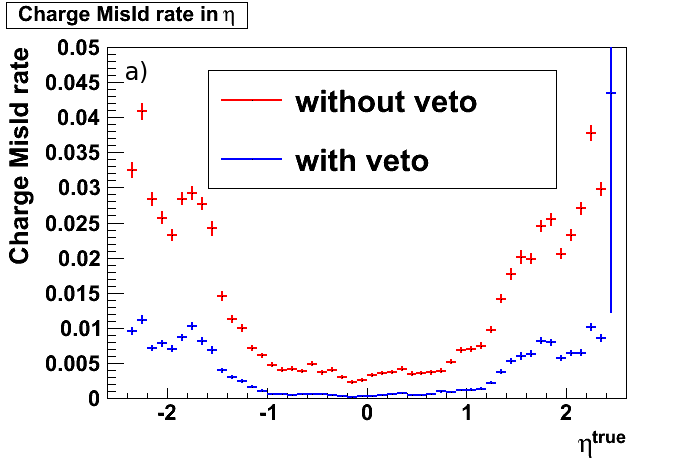
\includegraphics[width=0.485\linewidth,height=0.37\linewidth]{figs/ChargeMisIdRateEta.png}
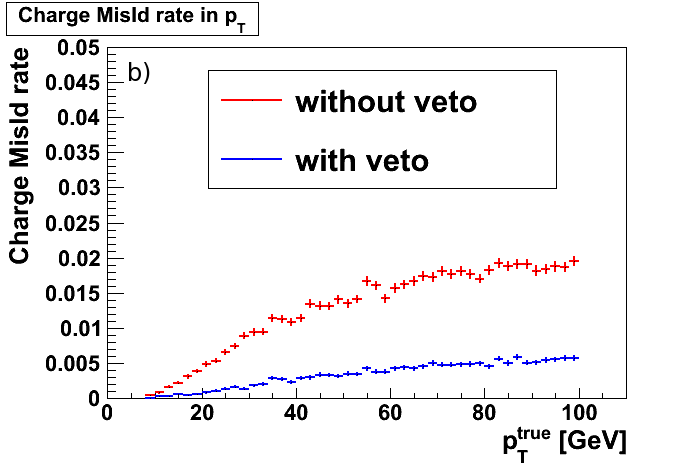
\includegraphics[width=0.485\linewidth,height=0.37\linewidth]{figs/ChargeMisIdRatePt.png}
\caption{Charge mis-identification rate, as a function of a) $\eta$ and b) $p_T$ of the generated
electron using ``electron gun'' sample \label{fig:charge_misid}. The solid (blue) distribution shows
the rate after the veto; if the reconstructed charge is not same for GSF and CTF tracks.}
\end{center}
\end{figure}

The GSF and GeneralTracks (CTF) are then associated based on sharing of the hits in the silicon strip tracking detector. 
The electrons are vetoed, if charge of the GSF track is not same as the charge of the associated 
GeneralTrack. Figure~\ref{fig:charge_misid} shows the charge mis-identification rate as a function of 
pseudorapidity ($\eta$) and transverse momentum ($p_T$) of the generated electron. The charge mis-identification rate
is reduced by factor of $\approx 3.9$, with a moderate ($2.1\%$)  loss in electron reconstruction efficiency after the veto. 
The rate after the veto is found to vary between $0.04\%$ to $1\%$ with increase in pseudorapidity. This selection is 
applied as part of the standard selection for rest of this document.

\section{Event Yields}
\label{sec:yields}

Applying the event selections described in Section~\ref{sec:eventselection}
to the Monte Carlo data sets described in Section~\ref{sec:datasamples}, 
results in the expected event yields in 100 pb$^{-1}$ listed 
in Table~\ref{tab:yields} and ~\ref{tab:yieldssusy} for SM and SUSY benchmark points, 
respectively.  

\begin{table}[hbt]
\begin{center}

\begin{tabular}{|l|c|c|c|c|c|c|c|c|}\hline
Same Sign leptons & Total SM & \ttbar & tW & WZ & ZZ & WW & DY & Wjets \\ \hline
 $ee$ & 0.45 & 0.44 & 0.00 & 0.00 & 0.01 & 0.00 & 0.00 & 0.00 \\
 $\mu\mu$ & 0.17 & 0.13 & 0.00 & 0.03 & 0.01 & 0.00 & 0.00 & 0.00 \\
 $e\mu$ & 0.48 & 0.39 & 0.04 & 0.04 & 0.01 & 0.00 & 0.00 & 0.00 \\
 total & 1.10 & 0.96 & 0.04 & 0.07 & 0.03 & 0.00 & 0.00 & 0.00 \\ \hline
\end{tabular}
\caption{Expected number of SM events passing the event selection in 100 pb$^{-1}$ of integrated 
luminosity.\label{tab:yields}}

\vspace{5 mm}

\begin{tabular}{|l|c|c|c|c|c|c|c|c|c|c|}\hline
Same Sign leptons & LM0 & LM1 & LM2 & LM3 & LM4 & LM5 & LM6 & LM7 & LM8 & LM9 \\ \hline
 $ee$ & 9.93 & 1.95 & 0.21 &1.45 & 0.49 & 0.17 & 0.45 & 0.22 & 0.72 & 0.50 \\
 $\mu\mu$ & 11.99 & 2.42 & 0.30 & 1.91 & 0.63 & 0.18 & 0.45 & 0.27 & 0.88 & 0.64 \\
 $e\mu$ & 22.52 & 4.55 & 0.48 & 3.09 & 1.18 & 0.34 & 0.86 & 0.42 & 1.62 & 1.26 \\
 total & 44.44 & 8.92 & 0.99 & 6.45 & 2.3 & 0.69 & 1.76 & 0.91 & 3.22 & 2.40 \\ \hline
\end{tabular}
\caption{Expected number of SUSY benchmark simulated events  passing the event selection in 100 pb$^{-1}$ of integrated 
luminosity.\label{tab:yieldssusy}}

\end{center}
\end{table}
This event selection shows a reasonable sensitivity to several SUSY points. 
The dominant contribution within SM is from \ttbar decays. 


\section{Discussion of backgrounds}
\label{sec:bkgtypes}

As shown in Section~\ref{sec:yields}, the SM background to this study is dominated 
by \ttbar events. The contribution from single-top, diboson production ($WZ, ZZ$), 
is small. The diboson backgrounds will be estimated from Monte Carlo. 
The Monte Carlo acceptances for these processes will be corrected for differences between 
data and Monte Carlo lepton identification and trigger efficiencies, as determined using 
the tag-and-probe method.

We study the same sign dileptons for the \ttbar background based on their origin.
The dominant source of dileptons in \ttbar events are produced via, $t \rightarrow W b$; where 
$W \rightarrow \ell \nu $. We classify them as follows, based on truth matched to their ``parents'':

\begin{itemize}
\item Type-I: both leptons originate from real $W$ (including $W \rightarrow \tau \rightarrow \ell$) bosons, one with mis-reconstructed charge.
\item Type-II a): one of the leptons is from a real $W$ and the other originates from heavy flavor sources ($b, c$).
\item Type-II b): one of the leptons is from a $W$ and the other is a fake lepton.
\item Type-III: both leptons are fakes or from heavy flavor sources.
\end{itemize} 

\begin{figure}[htb]
\begin{center}
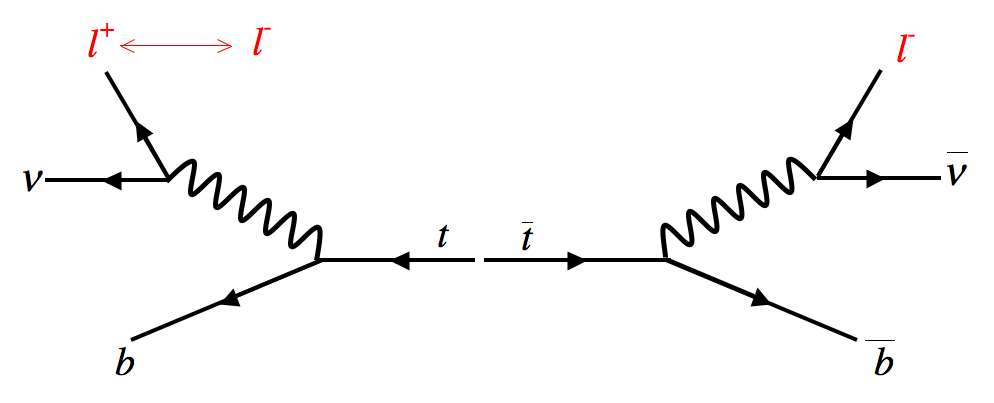
\includegraphics[width=0.32\linewidth, height=0.2\linewidth]{figs/feyntypeI.png}
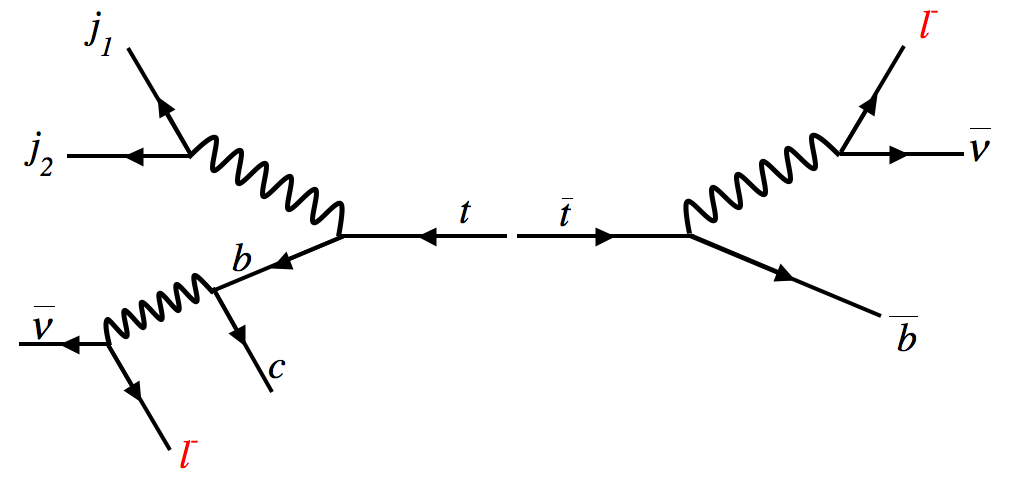
\includegraphics[width=0.32\linewidth, height=0.2\linewidth]{figs/feyntypeIIa.png}
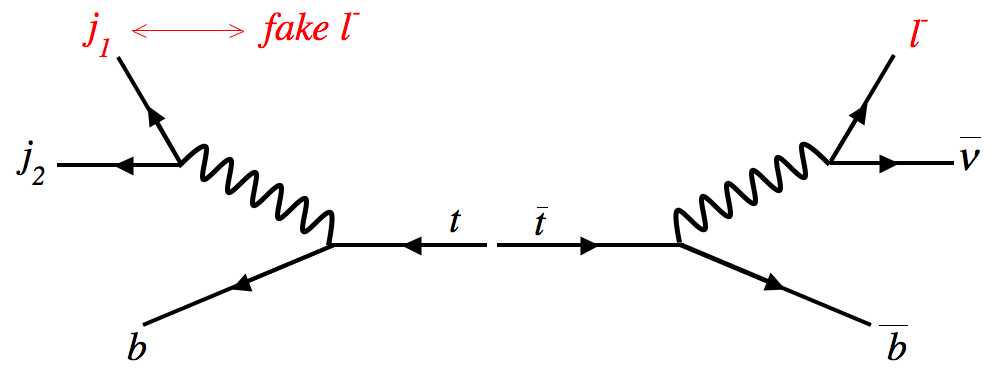
\includegraphics[width=0.32\linewidth, height=0.2\linewidth]{figs/feyntypeIIb.png}
\caption{ Classification of same sign dileptons from \ttbar decays. a) lepton from $W$ with mis-reconstructed charge; 
b) one of the lepton is from $W$, the other originating from heavy flavor sources; c) one of the lepton is from $W$,
and the other is a fake lepton. \label{fig:fakeOrigin}}
\end{center}
\end{figure}

Figure~\ref{fig:fakeOrigin} illustrates contribution from different types in \ttbar decays. The MC 
expectations of these contributions are given in Table~\ref{tab:fakeOrigin}.

\begin{table}[hbt]
\begin{center}
\begin{tabular}{|l|c|c|c|c|c|c|}\hline
Same Sign Leptons & Total & 	 Type-I &  Type-II & Type-II a) & Type-II b) & Type-III \\ \hline

$ee$ & 0.44$\pm$0.14 & 0.09$\pm$0.06 & 0.35$\pm$0.12 & 0.17$\pm$0.09 & 0.17$\pm$0.09 & 0.00$\pm$0.00 \\
$\mu\mu$ & 0.13$\pm$0.08 & 0.00$\pm$0.00 & 0.13$\pm$0.08 & 0.13$\pm$0.08 & 0.00$\pm$0.00 & 0.00$\pm$0.00 \\
$e\mu$ & 0.39$\pm$0.13 & 0.13$\pm$0.08 & 0.26$\pm$0.11 & 0.26$\pm$0.11 & 0.00$\pm$0.00 & 0.00$\pm$0.00 \\
total & 0.96$\pm$0.21 & 0.22$\pm$0.10 & 0.74$\pm$0.18 &	0.57$\pm$0.16 &	0.17$\pm$0.09 &	0.00$\pm$0.00 \\ \hline

\end{tabular}
\caption{ Expected number of \ttbar events of various types in 100 pb$^{-1}$ of integrated luminosity. Uncertainties are from MC statistics.\label{tab:fakeOrigin}}
\end{center}
\end{table}

It is interesting to note the following:
\begin{itemize}
\item Approximately $20 \%$, of the contribution is from Type-I (Charge mis-identification).
\item Almost all of the charge mis-identification is from electrons, in $ee$ and $e\mu$ channel.
\item The bulk of the \ttbar contribution in our event selection is from Type-II. The dominant among them 
is due to heavy flavor sources ($\sim 60 \%$)
\item No events with two fake leptons (Type-III) are expected within 100 pb$^{-1}$.
\end{itemize} 

In the following sections, we will briefly describe two different data driven approaches to 
estimate these contributions. The Type-I contribution will be estimated using the ``charge-flip rate'' described below, 
whereas the Type-II part will be estimated using the lepton fake rate method~\cite{fakelep}.




\section{Data driven method to estimate Charge Mis-Identification (Type-I)}
\label{sec:chargemisid}

The goal of the method is to predict, in a data driven way, the charge 
mis-identification of the electrons. This is accomplished
by measuring ``Charge-flip Rate'', $P_{ChargeFlip}$ using the Drell-Yan sample within the Z mass region
($76 < m_{ee} < 106 $ GeV). 

\subsection{Description of Charge-flip rate}

The method uses the probability of an electron to be reconstructed 
with a wrong charge as function of its $p_T$ and $\eta$.

\begin{equation}
P_{ChargeFlip} = \frac{N_{Wrong}(P_T, \eta)}{N_{Total}(P_T, \eta)}
\end{equation}

where $N_{Wrong}(P_T, \eta)$ is the number of wrongly charged electrons  and $N_{Total}(P_T, \eta)$ is 
the total number of electrons in the sample. We select events with same sign $(SS)$ 
and opposite sign $(OS)$ dielectrons within the $Z$ mass range. The number of wrongly 
charged electrons can be obtained:

\begin{equation}
  N_{Wrong}(P_T, \eta) = SS(P_T, \eta) - k(P_T, \eta) * OS(P_T, \eta) 
\end{equation}

The normalization $k(P_T, \eta)$ is given by the ratio of doubly charged $SS_{++/--}$ electrons to the 
admixture of a distribution of correctly charge-identified electrons and incorrectly-charge 
identified $OS$ electrons. The details of the procedure can be found in Ref.~\cite{chargefake}. 

In order to extrapolate to the $p_T$ and $\eta$ range covered by the \ttbar decays, we use a 
large ``electron gun'' MC. The Charge-flip rate is determined for the MC sample. The 
distribution is then validated to predict the charge-flip rate mentioned above 
using the Drell-Yan sample.

\begin{figure}[htb]
\begin{center}
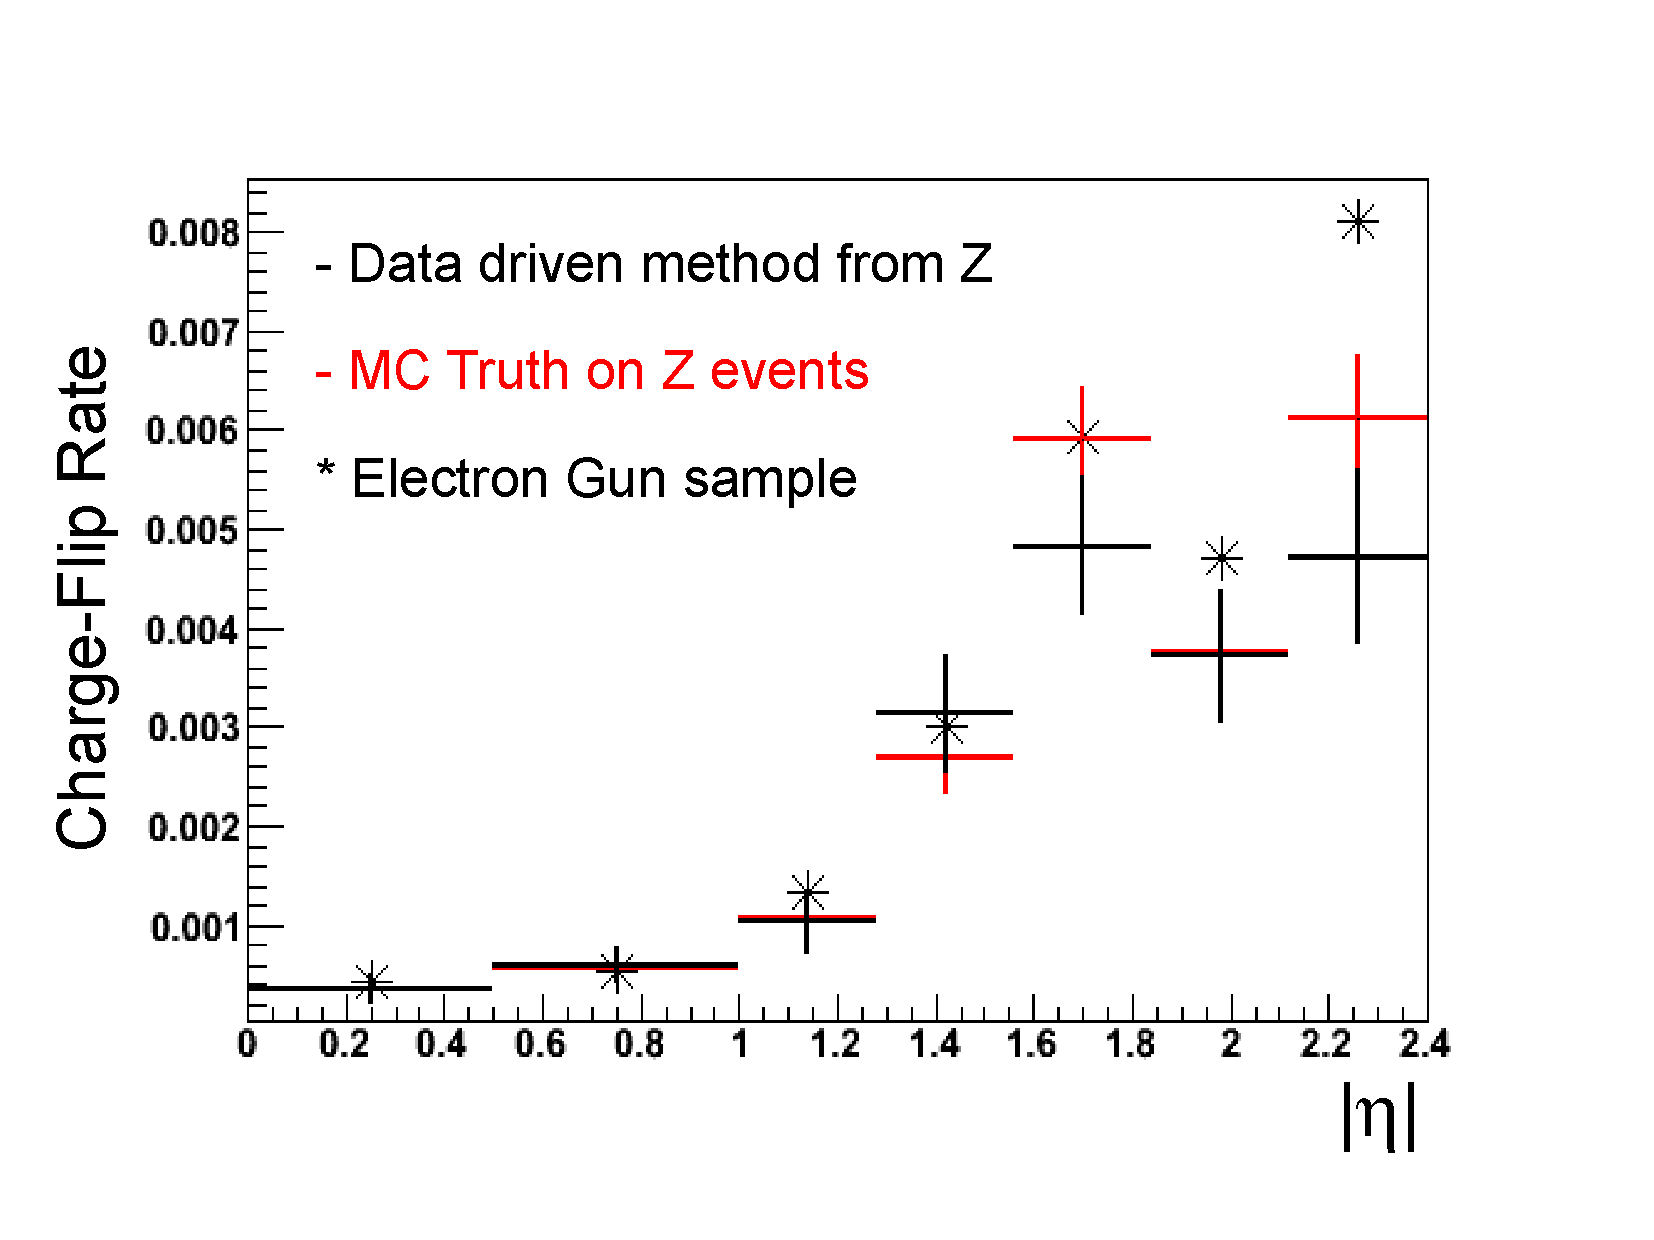
\includegraphics[width=0.7\linewidth]{figs/fr_rate.pdf}
\caption{Charge-flip rate as a function $|\eta|$ for the ``electron gun'' sample (star) compared with 
distributions using data driven method from $Z$ (black histograms) as well as truth matched $Z$ events 
(red histogram).\label{fig:charge_fliprate}}
\end{center}
\end{figure}

Figure~\ref{fig:charge_fliprate} shows the charge-flip rate as a function of $|\eta|$. The distribution from 
validated ``electron gun'' sample agree reasonably well with the expectation from data driven method
using $Z$ as well as MC truth matched $Z$ events. It should be noted that the charge-flip rate roughly 
reproduces the Charge mis-identification rate we observed earlier in Figure~\ref{fig:charge_misid} a).

\subsection{Application of Charge-flip rate to our analysis}

We now perform a rate test on \ttbar MC events by relaxing cuts on \met and jets. The test is meant
to demonstrate that the Charge-flip rate as determined from the ``electron gun'' sample can be applied
to \ttbar events. Dilepton events are selected without any \met and jet cuts using an integrated 
luminosity of 100 pb$^{-1}$. The observed event yield is obtained by selecting same sign electrons.
In order to get the estimation we use the following procedure:

\begin{itemize}
\item Select opposite sign dielectrons using the standard selection.
\item Obtain the $P^1_{ChargeFlip}$ and  $P^2_{ChargeFlip}$ for each electron for a given $p_T$ and $\eta$.
\item Assuming either of the electrons can flip signs, the flip probability is given by $ F = P_{ChargeFlip}/(1 - P_{ChargeFlip})$.
\item Weight each event by $weight * (F^1 + F^2)$.
\item Add up all of the weights
\end{itemize} 
Results of the Monte Carlo tests for event yields is given in Tables~\ref{tab:ChFlip_Test}. From this study we 
can conclude that the Charge-flip rate does a very good job of reproducing the rate of charge mis-identification
of electrons in \ttbar events.  
\begin{table}[hbt]
\begin{center}
\begin{tabular}{|l|c|}\hline
Sample & Event yield \\ \hline
\ttbar (Observed) & 2.4 $\pm$ 0.3 \\
\ttbar (Predicted) & 2.1 \\
\hline
\end{tabular}
\caption{ Monte Carlo test of the electron Charge-flip rate. \label{tab:ChFlip_Test}}
\end{center}
\end{table}

We are now ready to apply the Charge-flip rate to our \ttbar sample. The same sign dilepton sample will have 
three different contributions from Type-I, Type-II and Type-III events. The results of the application of 
the procedure outlined above is summarized in Table~\ref{tab:ChFakePredict}.
\vspace{2mm}
\begin{table}[hbt]
\begin{center}
\begin{tabular}{|l|c|c|c|c|c|c|}\hline
Same Sign leptons & Total &      Type-I &  Type-II & Type-II a) & Type-II b) & Type-III \\ \hline
$ee$ (predicted) 	 & 0.05 & 	0.05 &	0.00 &	0.00 &	0.00 &	0.00 \\
$\mu\mu$ (predicted)     & 0.00 &	0.00 &	0.00 &	0.00 &	0.00 &	0.00 \\
$e\mu$ (predicted)	 & 0.07 &	0.07 &	0.00 &	0.00 &	0.00 &	0.00 \\
total (predicted) 	 & 0.12 &	0.12 &	0.00 &	0.00 &	0.00 &	0.00 \\
\hline
\end{tabular}
\caption{ The number of events predicted using Charge-flip rate in \ttbar events for various types. Rates are normalized 
to 100 pb$^{-1}$.\label{tab:ChFakePredict}}
\end{center}
\end{table}

Using Table~\ref{tab:fakeOrigin} as observed and Table~\ref{tab:ChFakePredict} as the 
prediction, we find that the Charge-flip method predicts the bulk of the Type-I events. As expected,
the method does not predict any contribution from Type-II events. 
We consider the agreement quite satisfactory.
%This is quite satisfactory
%assuming a large systematic uncertainty are involved on these predictions.


\section{Data driven Method for Fake Lepton backgrounds (Type-II)}
\label{sec:leptonfake}

In this analysis, the primary source of events are from Type-II category. 
As shown in Table~\ref{tab:fakeOrigin}, roughly 3/4 of these events are expected to be from 
heavy flavor sources, while the remainder is from
fake leptons (Type-II b)). This means that one needs to be careful in defining the lepton fake rates
to make sure they predict both sources of fakes with sufficient accuracy.

In Reference~\cite{fakelep} we described a data-driven method to predict the fake 
background in a dilepton analysis. This method is being applied by us also 
in the WW~\cite{ww} as well as \ttbar ~\cite{ttbar} analyses. Here we briefly
summarize the method, and we apply it to the same sign dilepton study.

\subsection{The fake rate definition}
\label{subsec:fakeratedef}

The method starts by defining a fake rate ($FR$) measured in QCD events. We use 
the Pythia QCD samples with $\hat{P_T} > 30, 80 $ GeV. The fake rate is defined as 
the probability for a lepton passing loose cuts (Fakeable Object, $FO$) to pass the 
analysis cuts as a function of $p_T$ and $\eta$. The measured probability is then applied to 
dilepton candidates passing loose cuts to obtain a prediction to the fake lepton contribution. 
The details of the applications of the $FR$ are given in Section~\ref{subsec:fakerateapplication}. 

Fakeable Objects are defined as follows:

\begin{itemize}
\item Electron Fakeable Object, $eFO$:
\begin{itemize}
\item GSFElectron with $p_T > 10$ GeV;
\item $|\eta| < 2.4$;
\item No reconstructed muon with $\Delta R < 0.1$;
\item Electron ID and Conversion rejection defined in Section~\ref{sec:electron} as well as veto used in Section~\ref{sec:gsfctf};
\item Iso $<$ 0.4, where Iso=Sum/Max(20 GeV, $P_T$), and Sum = tkIso + hcalIso +  Max(0 GeV, ecalIso - 2 GeV).
\end{itemize} 

\item Muon Fakeable Object, $\mu FO$:
\begin{itemize}
\item Global and Tracker Muon with $p_T > 10$ GeV;
\item $|\eta| < 2.4$;
\item Global fit $\chi^2 /$ndof $ < 20 $;
\item $|d_0| < 200~\mu m$ (from silicon track, corrected for beamspot);
\item Iso $<$ 0.4, where Iso=Sum/Max(20 GeV, $P_T$), and Sum = tkIso + hcalIso +  ecalIso.
\end{itemize} 
\end{itemize} 

The $FR$ for electrons and muons are determined from the QCD sample.
% are shown in Figure.xx [Need a figure]
The $FR$ does not give a direct measure for an absolute lepton fake rate. It is the probability for a
fake lepton passing loose identification requirements as well as isolation to also pass a tighter
selection. 

\subsection{Application of lepton fake rate to our analysis}
\label{subsec:fakerateapplication}

We evaluate the $FR$ in \ttbar Monte Carlo events. This test is meant to check if the 
$FR$ as determined from the QCD events can be applied to \ttbar. In order to perform this test we 
define the following four event selections:

\begin{itemize}
\item \ttbar $\rightarrow Wb Wb \rightarrow \mu + e$  $ \nu \nu b b$:
\begin{itemize}
  \item Require a global muon with $p_T > 10$ GeV, truth matched to $W \rightarrow \mu$.
  \item Require a same sign electron that passes all the standard identification and isolation requirements. 
\end{itemize} 

\item \ttbar $\rightarrow Wb Wb \rightarrow \mu + (eFO \times FR)$  $ \nu \nu b b$:
\begin{itemize}
  \item Require a global muon with $p_T > 10$ GeV, truth matched to $W \rightarrow \mu$.
  \item Require a same sign $eFO$; weight each event by the $FR$ for the corresponding $eFO$.
\end{itemize} 

\item \ttbar $\rightarrow Wb Wb \rightarrow e + \mu  $  $ \nu \nu b b$:
\begin{itemize}
  \item Require an electron with $p_T > 10$ GeV, truth matched to $W \rightarrow e$.
  \item Require a same sign muon that passes all the standard identification and isolation requirements. 
\end{itemize} 

\item \ttbar $\rightarrow Wb Wb \rightarrow e + (\mu FO \times  FR)$  $ \nu \nu b b$:
\begin{itemize}
  \item Require an electron with $p_T > 10$ GeV, truth matched to $W \rightarrow e$.
  \item Require a same sign $\mu FO$; weight each event by the $FR$ for the corresponding $\mu FO$.
\end{itemize} 
\end{itemize} 

\begin{table}[hbt]
\begin{center}
\begin{tabular}{|l|c|}\hline
Sample & Event yield \\ \hline
\ttbar with $\mu + e$ (Observed) & 2.1 $\pm$ 0.3 \\
\ttbar with $\mu + (eFO \times FR)$ (Predicted) & 2.9 \\
\hline
\end{tabular}
\caption{ Monte Carlo test of the electron fake rate using 100 pb$^{-1}$ of integrated luminosity. \label{tab:EleFR_Test}}
\end{center}
\end{table}
\begin{table}[hbt]
\begin{center}
\begin{tabular}{|l|c|}\hline
Sample & Event yield \\ \hline
\ttbar with $e + \mu$ (Observed) & 2.4 $\pm$ 0.3 \\
\ttbar with $e + (\mu FO \times FR)$ (Predicted) & 2.7 \\
\hline
\end{tabular}
\caption{ Monte Carlo test of the muon fake rate using 100 pb$^{-1}$ of integrated luminosity. \label{tab:MuonFR_Test}}
\end{center}
\end{table}

The Monte Carlo test for the electron $FR$ consists of comparing event yields and distributions for 
$\mu + e $ and $\mu + (eFO \times FR)$. Similarly, for muon $FR$ it consists of comparing event yields 
and distributions for $ e + \mu$  and $e + (\mu DO \times FR)$. 
Results of the Monte Carlo tests for event yields are given in Tables~\ref{tab:EleFR_Test} and~\ref{tab:MuonFR_Test}.
The uncertainties are from the MC statistics. From these studies we conclude that the QCD $FR$ parametrization 
does a good job of reproducing the rate of fake electrons and muons in \ttbar events.

In order to obtain a prediction of the fake contribution to our analysis, we proceed in the following way:
\begin{itemize}
\item Select lepton $+ FO$ events where
\begin{itemize}
  \item one of the leptons passes all the standard identification and isolation requirements.
  \item the other lepton is a $FO$ but fails the standard identification and isolation requirements.
\end{itemize} 
\item The event passes all the standard kinematical cuts as outlined in Section~\ref{sec:eventselection}
\item Weigh each event by $FR/(1 - FR)$, where $FR$ is the fake rate for the $FO$ under consideration.
\item Add up all the weights.
\end{itemize} 

\vspace{2mm}
\begin{table}[hbt]
\begin{center}
\begin{tabular}{|l|c|c|c|c|c|c|}\hline
Same Sign leptons & Total &      Type-I &  Type-II & Type-II a) & Type-II b) & Type-III \\ \hline
$ee$ (predicted) &	0.21 &	0.01 &	0.20 &	0.15 &	0.05 &	0.00 \\
$\mu\mu$ (predicted) &	0.10 &	0.00 &	0.10 &	0.09 &	0.01 &	0.00 \\
$e\mu$ (predicted) &	0.31 &	0.01 &	0.30 &	0.26 &	0.04 &	0.00 \\
total (predicted) &	0.62 &	0.02 &	0.60 &	0.50 &	0.10 &	0.00 \\
\hline
\end{tabular}
\caption{ The number of events predicted using lepton fake rate method in \ttbar events for various types. 
Rates are normalized to 100 pb$^{-1}$.\label{tab:LeptonFakePredict}}
\end{center}
\end{table}
 The results of the application of the procedure outlined above is summarized in Table~\ref{tab:LeptonFakePredict}. 
We conclude the following in comparison with the observed events from Table~\ref{tab:fakeOrigin}:


\begin{itemize}
\item We predict within $\sim 20 \%$ of the observed Type-II contributions.
\item Within Type-II, the contribution from events with heavy flavor sources are largely predicted ($\sim 88 \%$).
\item The method introduces an overestimate for the true leptons in Type-I. This is at $\sim 2 \%$ level, 
this is negligible compared to the associated statistical as well as systematic uncertainties.
\end{itemize}

\section{Application of the data driven methods to the SM and SUSY benchmark points}
\label{sec:application}
We apply the two data driven procedures to predict the backgrounds in the 
\ttbar-dominated SM sample. Table~\ref{tab:yieldsObsPre} shows the contribution 
of all SM background. The prediction and observation agree to within $\sim 30\%$.

\begin{table}[hbt]
\begin{center}
\begin{tabular}{|l|c|c|c|c|c|c|c|c|}\hline
Same Sign leptons & Total SM & \ttbar & tW & WZ & ZZ & WW & DY & Wjets \\ \hline
 $ee$ (observed) & 0.45 & 0.44 & 0.00 & 0.00 & 0.01 & 0.00 & 0.00 & 0.00 \\
 $ee$ (predicted) & 0.27 & 0.26 & 0.01 & 0.00 & 0.00 & 0.00 & 0.00 & 0.00 \\ \hline	
 $\mu\mu$ (observed) & 0.17 & 0.13 & 0.00 & 0.03 & 0.01 & 0.00 & 0.00 & 0.00 \\
 $\mu\mu$ (predicted) & 0.11 & 0.10 & 0.01 & 0.00 & 0.00 & 0.00 & 0.00 & 0.00 \\ \hline
 $e\mu$ (observed) & 0.48 & 0.39 & 0.04 & 0.04 & 0.01 & 0.00 & 0.00 & 0.00 \\
$e\mu$ (predicted) & 0.39 & 0.38 & 0.01 & 0.00 & 0.00 & 0.00 & 0.00 & 0.00 \\ \hline	
 total (observed) & 1.10 & 0.96 & 0.04 & 0.07 & 0.03 & 0.00 & 0.00 & 0.00 \\ 
total (predicted) & 0.77 & 0.74 & 0.03 & 0.00 & 0.00 & 0.00 & 0.00 & 0.00 \\ \hline
\end{tabular}
\caption{Observed and predicted  number of SM events passing the event selection in 100 pb$^{-1}$ of integrated
luminosity.\label{tab:yieldsObsPre}}
\end{center}
\end{table}

We also apply both of these methods to combination of SM and SUSY samples to derive the
prediction. Table~\ref{tab:yieldsSUSY}, show the contribution of observed and expected prediction to 
the sample. Typically one would compare observed with the prediction to look for excess 
in ``signal'' over the total background.
\begin{table}[hbt]
\begin{center}
\small\addtolength{\tabcolsep}{-5pt}
\begin{tabular}{|l|c|c|c|c|c|c|c|c|c|c|}\hline
Same Sign  & SM+LM0 & SM+LM1 & SM+LM2 & SM+LM3 & SM+LM4 & SM+LM5 & SM+LM6 & SM+LM7 & SM+LM8 & SM+LM9 \\ \hline
Observed & 45.54 & 10.02 & 2.09 & 7.55 & 3.4 &	1.79 &	2.86 &	2.01 &	4.32 &	3.50 \\ \hline
Predicted & 4.10 & 1.26 & 0.83 & 1.24 &	0.91 &	0.81 &	0.84 &	0.83 &	1.03 &	1.00 \\ \hline
\end{tabular}
\caption{Observed and predicted  number of SM and SUSY events passing the event selection in 100 pb$^{-1}$ of integrated
luminosity.\label{tab:yieldsSUSY}}
\end{center}
\end{table}
The associated systematic uncertainties are not discussed in this document. We plan to measure
them in data. Overall, the sources of systematics can be categorized as detector effects, effects 
of modeling of the contributing processes, uncertainties of the data-driven background 
prediction methods.  Systematic uncertainties from the lepton selection, ID, and reconstruction efficiencies will be
estimated based on the corresponding systematics of the tag-and-probe method used to determine these efficiencies 
$Z \rightarrow \ell \ell$ in data. We will assess the uncertainty arising from the jet energy scale
using $\gamma/Z$ balance with jets. The uncertainties of the data-driven background estimate will be studied using 
a measure of ``bias per lepton'' as a function of the either charge fake candidate in charge-flip rate or $FO$ in
lepton fake rate selections. The current document focuses on reducing and measuring SM backgrounds using the aforesaid
data driven methods.

\clearpage

\section{Conclusion}
\label{sec:conclusion}
We have studied two different data driven methods to predict the backgrounds for  
searches beyond standard model, in events with high $P_T$ same sign dileptons
($e$ or $\mu$), significant hadronic activity, and high \met~. 
For these searches, the dominant background is from \ttbar. We characterized
the background into different types based on charge mis-identification,
leptons from heavy flavor sources, as well as fake leptons.

We used the charge-flip rate method to predict the wrongly charged 
leptons. The fakes including leptons from heavy flavor sources are predicted 
using lepton fake rates. Using both the methods to the entire ensemble of the
SM as well as SUSY samples, we show sensitivity towards several SUSY benchmark 
points using 100 pb$^{-1}$ of integrated luminosity.




\clearpage
\begin{thebibliography}{99}

\bibitem{tosi}{\tt http://www.ge.infn.it/\~tosi/cms/topMC.html}.

\bibitem{summer08} {\tt https://twiki.cern.ch/twiki/bin/view/CMS/ProductionSummer2008}.

\bibitem{ww} {``Prospects for measuring the $WW$ production cross section in $pp$ collisions at $\sqrt s = $10 TeV''}, CMS AN-2009/042 and PAS EWK-09-002.

\bibitem{ttbar} {``Expectations for observation of top quark pair production in the dilepton final state with the early CMS data''}, CMS AN-2009/050 and PAS TOP-09-002.

\bibitem{tcmet} {``Correcting Missing Transverse Energy Using Tracks''}, CMS AN-2009/022.

\bibitem{conversion} {\tt http://indico.cern.ch/materialDisplay.py?contribId=3\&materialId=slides\&confId=58309}.

\bibitem{glbtrk} {\tt https://hypernews.cern.ch/HyperNews/CMS/get/muon/258.html}.

\bibitem{muonid} {``Muon Identification in CMS''}, CMS AN-2008/098.

\bibitem{vplusj} {\tt https://twiki.cern.ch/twiki/bin/view/CMS/VplusJets}.

\bibitem{ctfgsf} {\tt http://indico.cern.ch/materialDisplay.py?contribId=3\&materialId=slides\&confId=64436}.

\bibitem{fakelep} {``Data-driven methods to estimate the electron and muon fake contributions to lepton analyses''}, CMS AN-2009/041.

\bibitem{chargefake} P. Kalavase, et. al, Analysis Note in preparation.

\end{thebibliography}









\end{document}
